\documentclass{article} 

\usepackage[brazil]{babel}
\usepackage{enumitem}
\usepackage{amsmath}
\usepackage{booktabs}
\usepackage{bm}
\usepackage{float}
\usepackage[margin=2cm]{geometry}
\usepackage{circuitikz}
\usepackage{siunitx}
\usepackage{steinmetz}
\usepackage{amssymb}

\newcommand{\phasor}[2]{%
  #1 \, \phase{\, #2^\circ} \,
}

\newcommand{\ds}{\displaystyle}

% \newcommand{\phasor}[2]{%
%   #1 \, \text{\phase{\, \ang{#2}}} \,
% }

\newcommand{\nle}{%
  \notag \\[0pt]
}

\setlength{\parindent}{0pt}

\title{Modelagem Matemática da Microrrede CC} 
\author{} 
% \date{\today}
\date{}

\begin{document}

\maketitle

\section*{Esquemático da Microrrede}

\begin{figure}[h]
  \centering
  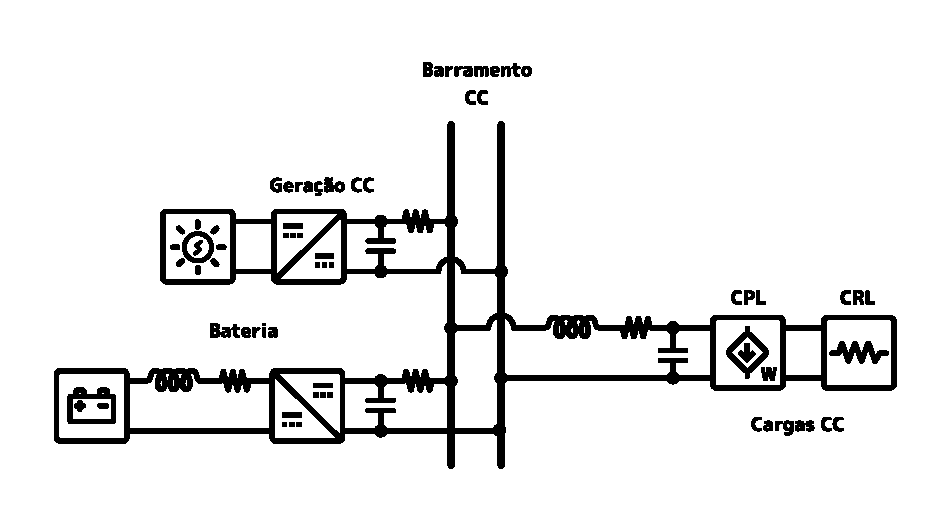
\includegraphics[scale=1.]{assets/dc_microgrid.eps}
  \caption{Esquemático da Microrrede CC}
  \label{fig:exemplo}
\end{figure}

\subsection*{Modelagem do Subsistema: Geração 1}

O sistema da geração 1, apresentado na Figura~\ref{fig:subsystem_1},  é composto por uma fonte de alimentação cuja tensão varia ao longo do tempo, a qual está conectada a um conversor do tipo {\it buck}. Este conversor, por sua vez, está ligado a um filtro RC. Finalmente, o conjunto é conectado ao barramento de corrente contínua (CC).

\begin{figure}[H]
  \centering
  \begin{circuitikz}[american, scale=0.5, font=\footnotesize]
    \ctikzset{bipoles/length=1cm}
    \draw
    (0,4) to[vsource, v_=$v_{\text{in}, 1}(t)$] (0,0)
    (0,4) to[normal open switch, l=$S_1$] (4,4)
    (4,0) to[diode, l=$D_1$] (4,4)
    (4,4) to[L, l=$L_1$, i_=$i_{L,1}(t)$] (8,4)
    (7,4) to[R, l=$R_{1,1}$] (11,4)
    (11,4) to[C, l=$C_1$, v=$v_{C,1}(t)$] (11,0)
    (11,4) to[R, l=$R_{1,2}$, i_=$i_{E,1}(t)$] (15,4)
    
    (15,4) to[short, -o] (16,4)
    (0,0) to[short, -o] (16,0)
    
    (16,4) to[open, v=$v_E(t)$] (16,0)
    ;
  \end{circuitikz}
  \caption{Circuito elétrico do sistema da geração 1.}
  \label{fig:subsystem_1}
\end{figure}

Aplicando a LKT na segunda malha a partir da esquerda, obtemos:
\begin{gather}
  d_1(t) v_{\text{in}, 1}(t) - L_1 \dot{i}_{L,1} - R_{1,1} i_{L,1}(t) - v_{C,1}(t) = 0 \nle
  \dot{i}_{L,1} = - \frac{R_{1,1}}{L_1} i_{L,1}(t) - \frac{1}{L_1} v_{C,1}(t) + \frac{v_{\text{in}, 1}(t)}{L_1} d_1(t)
\end{gather}

Aplicando a LKC, obtemos:
\begin{gather}
  i_{L,1}(t) = C_1 \dot{v}_{C,1} + i_{E,1}(t)
\end{gather}

Têm-se que, $i_{E,1}(t) = \ds \frac{v_{C,1}(t) - v_E(t)}{R_{1,2}}$. Logo,
\begin{gather}
  i_{L,1}(t) = C_1 \dot{v}_{C,1} + \frac{1}{R_{1,2}}v_{C,1}(t) - \frac{1}{R_{1,2}} v_E(t) \nle
  i_{L,1}(t) = C_1 \dot{v}_{C,1} + \frac{1}{R_{1,2}}v_{C,1}(t) - \frac{1}{R_{1,2}} v_E(t) \nle
  \dot{v}_{C,1} = \frac{1}{C_1} i_{L,1}(t) - \frac{1}{R_{1,2}C_1 }v_{C,1}(t) + \frac{1}{R_{1,2} C_1} v_E(t)
\end{gather}

Portanto, o modelo do subsistema da geração é:
\begin{gather}
  \begin{cases}
    \dot{i}_{L,1} = \ds - \frac{R_{1,1}}{L_1} i_{L,1}(t) - \frac{1}{L_1} v_{C,1}(t) + \frac{v_{\text{in}, 1}(t)}{L_1} d_1(t) \\[12pt]
    \dot{v}_{C,1} = \ds \frac{1}{C_1} i_{L,1}(t) - \frac{1}{R_{1,2}C_1 }v_{C,1}(t) + \frac{1}{R_{1,2} C_1} v_E(t)
  \end{cases}
\end{gather}

\vspace*{8pt}
\subsection*{Modelagem do Subsistema: Conversor Boost}

O sistema da geração 2, apresentado na Figura~\ref{fig:subsystem_2},  é composto por uma fonte de alimentação cuja tensão varia ao longo do tempo, a qual está conectada a um conversor do tipo {\it boost}. Este conversor, por sua vez, está ligado a um filtro RC. Finalmente, o conjunto é conectado ao barramento de corrente contínua (CC).

\begin{figure}[H]
  \centering
  \begin{circuitikz}[american, scale=0.5, font=\footnotesize]
    \ctikzset{bipoles/length=1cm}
    \draw
    (-4,4) to[vsource, v_=$v_{\text{in}, 2}(t)$] (-4,0)
    (-4,4) to[R, l=$R_{2,1}$, i_=$i_{L,2}$] (0,4)
    (0,4) to[L, l=$L_2$] (4,4)
    (4,0) to[normal open switch, l=$S_2$] (4,4)
    (4,4) to[diode, l=$D_2$] (8,4)
    (8,4) to[C, v=$v_{C,2}$, l=$C_2$] (8,0)
    (8,4) to[R, l=$R_{2,2}$, -o, i=$i_{E,2}$] (12,4)
    (-4,0) to[short, -o] (12,0)
    (12,4) to[open, v=$v_E$] (12,0)
    ;
  \end{circuitikz}
  \caption{Circuito elétrico do sistema da geração 2.}
  \label{fig:subsystem_2}
\end{figure}

\subsubsection*{Para $S_2$ fechada: $d_2(t) \cdot T_s$}

Aplicando a LKT na malha mais a esquerda, obtemos:
\begin{gather}
  v_{\text{in}, 2}(t) - R_{2,1} i_{L,2}(t) - L_2 \dot i_{L,2} = 0  \nle
  \dot i_{L,2} = - \frac{R_{2,1}}{L_2} i_{L,2}(t) + \frac{1}{L_2} v_{\textit{in}, 2}(t)
\end{gather}

Aplicando a LKC na malha mais a direita, tém-se:
\begin{gather}
  i_{E,2}(t) + C_2 \dot{v}_{C,2} = 0
\end{gather}

Como $i_{E,2}(t) = \ds \frac{v_{C,2}(t) - v_E(t)}{R_{2,2}}$, têm-se:
\begin{gather}
  \frac{v_{C,2}(t)}{R_{B,2}} - \frac{v_E(t)}{R_{B,2}} + C_2 \dot{v}_{C,2} = 0 \nle
  \dot{v}_{C,2} = - \frac{1}{R_{B,2} C_2} v_{C,2}(t) + \frac{1}{R_{B,2} C_2} v_{E}(t)
\end{gather}

Assim, neste modo, têm-se:
\begin{gather}
  \begin{cases}
    \dot i_{L,2} = \ds - \frac{R_{2,1}}{L_2} i_{L,2}(t) + \frac{1}{L_2} v_{\textit{in}, 2}(t) \\[12pt]
    \dot{v}_{C,2} = \ds - \frac{1}{R_{B,2} C_2} v_{C,2}(t) + \frac{1}{R_{B,2} C_2} v_{E}(t)
  \end{cases}
\end{gather}

\vspace*{8pt}
\subsubsection*{Para $S_2$ aberta: $\left[1 - d_2(t)\right] \cdot T_s$}

Aplicando a LKT, obtemos:
\begin{gather}
  v_{\text{in}, 2}(t) - L_2 \dot i_{L,2} - R_{2,1} i_{L,2} (t) - v_{C,2} (t)= 0 \nle
  \dot i_{L,2} = - \frac{R_{2,1}}{L_2} i_{L,2}(t) - \frac{1}{L_2} v_{C,2}(t) + \frac{1}{L_2} v_{\text{in}, 2}(t)
\end{gather}

Aplicando a LKC, obtemos:
\begin{gather}
  i_{L,2}(t) = C_2 \dot v_{C,2} + i_{E,2}(t) \nle
  i_{L,2}(t) = C_2 \dot v_{C,2} +  \frac{v_{C,2}(t)}{R_{2,2}} - \frac{v_E(t)}{R_{2,2}} \nle
  \dot{v}_{C,2} =  \frac{1}{C_2} i_{L,2}(t) - \frac{1}{R_{2,2}C_2} v_{C,2}(t) + \frac{1}{R_{2,2} C_2} v_E(t)
\end{gather}

Assim, neste modo, têm-se:
\begin{gather}
  \begin{cases}
    \dot i_{L,2} = \ds - \frac{R_{2,1}}{L_2} i_{L,2}(t) - \frac{1}{L_2} v_{C,2}(t) + \frac{1}{L_2} v_{\text{in}, 2}(t) \\[12pt]
    \dot{v}_{C,2} = \ds \frac{1}{C_2} i_{L,2}(t) - \frac{1}{R_{2,2}C_2} v_{C,2}(t) + \frac{1}{R_{2,2} C_2} v_E(t)
  \end{cases}
\end{gather}

\vspace*{8pt}
\subsubsection*{Modelo Médio Completo}
A equação completa da dinâmica da corrente ${i}_{L,2}(t)$ é:
\begin{gather}
  \dot{i}_{L,2} = \left[- \frac{R_{2,1}}{L_2} i_{L,2}(t) + \frac{1}{L_2} v_{\textit{in}, 2}(t)\right] d_2(t) + \left[- \frac{R_{2,1}}{L_2} i_{L,2}(t) - \frac{1}{L_2} v_{C,2}(t) + \frac{1}{L_2} v_{\text{in}, 2}(t)\right] \left[1 - d_2(t)\right] \nle
  \dot{i}_{L,2} = - \frac{R_{2,1}}{L_2} i_{L,2}(t) - \frac{1}{L_2} v_{C,2}(t) \left[1 - d_2(t)\right] + \frac{1}{L_2} v_{\text{in}, 2}(t)
\end{gather}

E da tensão,
\begin{gather}
  \dot{v}_{C,2} = \left[- \frac{1}{R_{B,2} C_2} v_{C,2}(t) + \frac{1}{R_{B,2} C_2} v_{E}(t)\right] d_2(t) + \left[\frac{1}{C_2} i_{L,2}(t) - \frac{1}{R_{2,2} C_2} v_{C,2}(t) + \frac{1}{R_{2,2} C_2} v_E(t)\right] \left[1 - d_2(t)\right] \nle
  \dot{v}_{C,2} = \frac{1}{C_2} i_{L,2}(t) \left[1 - d_2(t)\right] - \frac{1}{R_{2,2} C_2} v_{C,2}(t) + \frac{1}{R_{2,2} C_2} v_E(t)
\end{gather}

Portanto, o modelo dinâmico do sistema da geração 2 é:
\begin{gather}
  \begin{cases}
    \dot{i}_{L,2} =\ds - \frac{R_{2,1}}{L_2} i_{L,2}(t) - \frac{1}{L_2} v_{C,2}(t) \left[1 - d_2(t)\right] + \frac{1}{L_2} v_{\text{in}, 2}(t) \\[12pt]
    \dot{v}_{C,2} =\ds \frac{1}{C_2} i_{L,2}(t) \left[1 - d_2(t)\right] - \frac{1}{R_{2,2} C_2} v_{C,2}(t) + \frac{1}{R_{2,2} C_2} v_E(t)
  \end{cases}
\end{gather}

\vspace*{8pt}
\subsection*{Modelagem do Subsistema: Cargas}

O circuito que representa as duas cargas conectadas a redes, a CPL e a CRL, é:

\begin{figure}[H]
  \centering
  \begin{circuitikz}[american, scale=0.5, font=\footnotesize]
    \ctikzset{bipoles/length=1cm}
    \draw
    (0,4) to[open, v_=$v_E(t)$, o-o] (0,0)
    (0,4) to[L,l=$L_{K}$, i_=$i_{L_K}(t)$] (4,4)
    (3,4) to[R,l=$R_{K}$] (7,4)
    (7,4) to[C, l=$C_{K}$, v=$v_{C_K}(t)$] (7,0)
    (11,4) to[controlled current source, l={$i(t) = \frac{P_{cpl}(t)}{v_{C_K}(t)}$}] (11,0)
    (0,0) to[short] (16,0)
    (7,4) to[short] (16,4)
    (16,4) to[R, l=$R_{rcl}$] (16,0)
    ;
  \end{circuitikz}
\end{figure}

Aplicando a LKT na malha mais a esquerda, têm-se:
\begin{gather}
  v_E(t) - L_K \dot{i}_{L_K} - R_K i_{L_K}(t) - v_{C_K}(t) = 0 \nle
  \dot{i}_{L_K} = - \frac{R_K}{L_K} i_{L_K}(t) - \frac{1}{L_K} v_{C_K}(t) + \frac{1}{L_K} v_E(t)
\end{gather}

Aplicando a LKC, obtemos:
\begin{gather}
  i_{L_K} = C_K \dot{v}_{C_K} + \frac{P_{cpl}(t)}{v_{C_K}(t)} + \frac{v_{C_K}(t)}{R_{crl}} \nle
  \dot{v}_{C_K} = \frac{1}{C_K} i_{L_K} - \frac{1}{R_{crl} C_K} v_{C_K}(t) - \frac{1}{C_K} \frac{P_{cpl}(t)}{v_{C_K}(t)}
\end{gather}

Portanto, o modelo dinâmico do subsistema das cargas é:
\begin{gather}
  \begin{cases}
    \dot{i}_{L_K} = \ds - \frac{R_K}{L_K} i_{L_K}(t) - \frac{1}{L_K} v_{C_K}(t) + \frac{1}{L_K} v_E(t) \\[12pt]
    \dot{v}_{C_K} = \ds \frac{1}{C_K} i_{L_K} - \frac{1}{R_{crl} C_K} v_{C_K}(t) - \frac{1}{C_K} \frac{P_{cpl}(t)}{v_{C_K}(t)}
  \end{cases}
\end{gather}

\subsection*{Centralização dos Modelos}

Do esquemático, têm-se que:
\begin{gather}
  i_{E,1}(t) + i_{E,2}(t) = i_B(t) + i_{L_K}(t) \nle
  \frac{1}{R_{1,2}} v_{C,1}(t) - \frac{1}{R_{1,2}} v_E(t) + \frac{1}{R_{2,2}} v_{C,2}(t) - \frac{1}{R_{2,2}} v_E(t) =
  i_B(t) + i_{L_K}(t) \nle
  v_E(t) = \frac{R_{EQ}}{R_{1,2}} v_{C,1}(t) + \frac{R_{EQ}}{R_{2,2}} v_{C,2}(t) - R_{EQ} i_B(t) - R_{EQ} i_{L_K}(t)
\end{gather}

onde, $R_{EQ} = \ds \frac{R_{1,2}R_{2,2}}{R_{1,2} + R_{2,2}}$.

\vspace*{8pt}

Reescrevendo a equação de $i_{L_K}$, obtêm-se:
\begin{gather}
  \dot{i}_{L_K} =  - \frac{R_K}{L_K} i_{L_K}(t) - \frac{1}{L_K} v_{C_K}(t) + \frac{1}{L_K} \left[\frac{R_{EQ}}{R_{1,2}} v_{C,1}(t) + \frac{R_{EQ}}{R_{2,2}} v_{C,2}(t) - R_{EQ} i_B(t) - R_{EQ} i_{L_K}(t)\right] \nle
  \dot{i}_{L_K} =  - \frac{R_K + R_{EQ}}{L_K} i_{L_K}(t) - \frac{1}{L_K} v_{C_K}(t) + \frac{R_{EQ}}{R_{1,2} L_K} v_{C,1}(t) + \frac{R_{EQ}}{R_{2,2} L_K} v_{C,2}(t) - \frac{R_{EQ}}{L_K} i_B(t)
\end{gather}

Reescrevendo a equação de $v_{C,1}$, obtêm-se:
\begin{gather*}
  \dot{v}_{C,1} = \frac{1}{C_1} i_{L,1}(t) - \frac{1}{R_{1,2}C_1} v_{C,1}(t) + \frac{1}{R_{1,2} C_1} \left[\frac{R_{EQ}}{R_{1,2}} v_{C,1}(t) + \frac{R_{EQ}}{R_{2,2}} v_{C,2}(t) - R_{EQ} i_B(t) - R_{EQ} i_{L_K}(t)\right]
\end{gather*}
\begin{gather}
  \dot{v}_{C,1} = \frac{1}{C_1} i_{L,1}(t) - \frac{1}{R_{1,2}C_1} \left(1  - \frac{R_{EQ}}{R_{1,2}}\right) v_{C,1}(t) +\frac{1}{C_1 (R_{1,2} + R_{2,2})} v_{C,2}(t) - \frac{R_{EQ}}{R_{1,2}C_1} i_B(t) - \frac{R_{EQ}}{R_{1,2}C_1} i_{L_K}(t)
\end{gather}

Reescrevendo a equação de $v_{C,2}$, obtêm-se:
\begin{gather*}
  \dot{v}_{C,2} = \frac{1}{C_2} i_{L,2}(t) \left[1 - d_2(t)\right] - \frac{1}{R_{2,2} C_2} v_{C,2}(t) + \frac{1}{R_{2,2} C_2} \left[\frac{R_{EQ}}{R_{1,2}} v_{C,1}(t) + \frac{R_{EQ}}{R_{2,2}} v_{C,2}(t) - R_{EQ} i_B(t) - R_{EQ} i_{L_K}(t)\right]
\end{gather*}
\begin{multline}
  \dot{v}_{C,2} = \frac{1}{C_2} \left[1 - d_2(t)\right] i_{L,2}(t)
  - \frac{1}{R_{2,2} C_2} \left(1 - \frac{R_{EQ}}{R_{2,2}}\right) v_{C,2}(t)\\
  + \frac{1}{C_2 (R_{1,2} + R_{2,2})} v_{C,1}(t)
  - \frac{R_{EQ}}{R_{2,2}C_2} i_B(t) - \frac{R_{EQ}}{R_{2,2}C_2} i_{L_K}(t)
\end{multline}

Assim, o modelo centralizado é:

\begin{gather}
  \begin{cases}
    \dot{i}_{L,1} = - \frac{R_{1,1}}{L_1} i_{L,1}(t) - \frac{1}{L_1} v_{C,1}(t) + \frac{v_{\text{in}, 1}(t)}{L_1} d_1(t)                                                                                                                        \\[12pt]
    \dot{v}_{C,1} = \frac{1}{C_1} i_{L,1}(t) - \frac{1}{R_{1,2}C_1} \left(1  - \frac{R_{EQ}}{R_{1,2}}\right) v_{C,1}(t) +\frac{1}{C_1 (R_{1,2} + R_{2,2})} v_{C,2}(t) - \frac{R_{EQ}}{R_{1,2}C_1} i_B(t) - \frac{R_{EQ}}{R_{1,2}C_1} i_{L_K}(t) \\[12pt]
    \dot{i}_{L,2} = - \frac{R_{2,1}}{L_2} i_{L,2}(t) - \frac{1}{L_2} v_{C,2}(t) \left[1 - d_2(t)\right] + \frac{1}{L_2} v_{\text{in}, 2}(t)                                                                                                     \\[12pt]
    \dot{v}_{C,2} = \frac{1}{C_2} \left[1 - d_2(t)\right] i_{L,2}(t)
    - \frac{1}{R_{2,2} C_2} \left(1 - \frac{R_{EQ}}{R_{2,2}}\right) v_{C,2}(t)
    + \frac{1}{C_2 (R_{1,2} + R_{2,2})} v_{C,1}(t)
    - \frac{R_{EQ}}{R_{2,2}C_2} i_B(t) - \frac{R_{EQ}}{R_{2,2}C_2} i_{L_K}(t)                                                                                                                                                              \\[12pt]
    \dot{i}_{L_K} = - \frac{R_K + R_{EQ}}{L_K} i_{L_K}(t) - \frac{1}{L_K} v_{C_K}(t) + \frac{R_{EQ}}{R_{1,2} L_K} v_{C,1}(t) + \frac{R_{EQ}}{R_{2,2} L_K} v_{C,2}(t) - \frac{R_{EQ}}{L_K} i_B(t)                                                \\[12pt]
    \dot{v}_{C_K} = \frac{1}{C_K} i_{L_K} - \frac{1}{R_{crl} C_K} v_{C_K}(t) - \frac{1}{C_K} \frac{P_{cpl}(t)}{v_{C_K}(t)}
  \end{cases}
\end{gather}


\subsection*{Translação do Modelo}

Parcelando os estados e as entradas do sistema em termos fixos e em termos variantes no tempo, obtemos:

\begin{align}
  i_{L,1}(t) & = i_{L,1}^o + \delta i_{L,1}(t) & i_{L,2}(t) & = i_{L,2}^o + \delta i_{L,2}(t) & i_{L_K}(t) & = i_{L_K}^o + \delta i_{L_K}(t) \nle
  v_{C,1}(t) & = v_{C,1}^o + \delta v_{C,1}(t) & v_{C,2}(t) & = v_{C,2}^o + \delta v_{C,2}(t) & v_{C_K}(t) & = v_{C_K}^o + \delta v_{C_K}(t) \nle
  d_1(t)     & = d_1^o + \delta d_1(t)         & d_2(t)     & = d_2^o + \delta d_2(t)         & P_{cpl}(t) & = P_{cpl}^o + \delta P_{cpl}(t) \nle
             &                                 & v_{\text{in},2}(t)     & = v_{\text{in},2}^o + \delta v_{\text{in},2}(t)         &            &
\end{align}

\textbf{\textit{Corrente $i_{L,1}$ transladada}} \vspace*{12pt}

Para $\dot{i}_{L,1}$, têm-se:
\begin{gather}
  - \frac{R_{1,1}}{L_1} i_{L,1}^o - \frac{1}{L_1} v_{C,1}^o + \frac{v_{\text{in}, 1}(t)}{L_1} d_1^o = 0 \Rightarrow
  - R_{1,1} i_{L,1}^o - v_{C,1}^o + v_{\text{in}, 1}(t) d_1^o = 0 \nle
  d_1^o = \frac{R_{1,1}}{v_{\text{in}, 1}(t)} i_{L,1}^o + \frac{1}{v_{\text{in}, 1}(t)} v_{C,1}^o
\end{gather}

Substituindo, obtemos:
\begin{gather}
  \dot{i}_{L,1} = - \frac{R_{1,1}}{L_1} i_{L,1}(t) - \frac{1}{L_1} v_{C,1}(t) + \frac{v_{\text{in}, 1}(t)}{L_1} d_1(t) \nle
  \delta \dot{i}_{L,1} = - \frac{R_{1,1}}{L_1} \left[i_{L,1}^o + \delta i_{L,1}(t)\right]
  - \frac{1}{L_1} \left[v_{C,1}^o + \delta v_{C,1}(t)\right]
  + \frac{v_{\text{in}, 1}(t)}{L_1} \left[\frac{R_{1,1}}{v_{\text{in}, 1}(t)} i_{L,1}^o + \frac{1}{v_{\text{in}, 1}(t)} v_{C,1}^o + \delta d_1(t)\right] \nle
  \delta \dot{i}_{L,1} = - \frac{R_{1,1}}{L_1} \delta i_{L,1}(t) - \frac{1}{L_1} \delta v_{C,1}(t) + \frac{v_{\text{in}, 1}(t)}{L_1} \delta d_1(t)
\end{gather}

\textbf{\textit{Corrente $i_{L,2}$ transladada}} \vspace*{12pt}

Para $\dot{i}_{L,2}$, têm-se:
\begin{gather}
  - \frac{R_{2,1}}{L_2} i_{L,2}^o - \frac{1}{L_2} \left[1 - d_2^o\right] v_{C,2}^o + \frac{1}{L_2} v_{\text{in},2}^o = 0 \Rightarrow
  d_2^o = 1 + \frac{R_{2,1}i_{L,2}^o}{v_{C,2}^o} - \frac{v_{\text{in},2}^o}{v_{C,2}^o}
\end{gather}

Substituindo, obtemos:
\begin{gather}
  \delta \dot{i}_{L,2} = - \frac{R_{2,1}}{L_2} \left[i_{L,2}^o + \delta i_{L,2}(t)\right] - \frac{1}{L_2} \left[1 - d_2^o - \delta d_2(t)\right] \left[v_{C,2}^o + \delta v_{C,2}(t)\right] + \frac{1}{L_2} \left[v_{\text{in},2}^o + \delta v_{\text{in},2}(t)\right] \nle
  \delta \dot{i}_{L,2} = \frac{R_{2,1}}{L_2} \delta i_{L,2}(t)
  + \left[\frac{R_{2,1} i_{L,2}^o}{L_2 v_{C,2}^o} - \frac{v_{\text{in},2}^o}{L_2 v_{C,2}^o}\right] \delta v_{C,2}(t) + \frac{1}{L_2} \left[v_{C,2}^o + \delta v_{C,2}(t)\right] \delta d_2(t) + \frac{1}{L_2} \delta v_{\text{in},2}(t)
\end{gather}

\textbf{\textit{Corrente $i_{L_K}$ transladada}} \vspace*{12pt}

Para $\dot{i}_{L_K}$, têm-se:
\begin{gather}
  - \frac{R_K + R_{EQ}}{L_K} i_{L_K}^o - \frac{1}{L_K} v_{C_K}^o + \frac{R_{EQ}}{{R_{1,2}}L_K} v_{C,1}^o + \frac{R_{EQ}}{R_{2,2}L_K} v_{C,2}^o - \frac{R_{EQ}}{L_K} i_B^o= 0 \nle
  v_{C,2}^o = \frac{R_{2,2}(R_K + R_{EQ})}{R_{EQ}} i_{L_K}^o + \frac{R_{2,2}}{R_{EQ}} v_{C_K}^o - \frac{R_{2,2}}{{R_{1,2}}} v_{C,1}^o + R_{2,2}i_B^o
\end{gather}

Substituindo, obtemos:
\begin{multline*}
  \delta \dot{i}_{L_K} = - \frac{R_K + R_{EQ}}{L_K} \left[i_{L_K}^o + \delta i_{L_K}(t)\right]
  - \frac{1}{L_K} \left[v_{C_K}^o + \delta v_{C_K}(t)\right] \\
  + \frac{R_{EQ}}{{R_{1,2}}L_K} \left[v_{C,1}^o + \delta v_{C,1}(t)\right]
  + \frac{R_{EQ}}{R_{2,2}L_K} \left[v_{C,2}^o + \delta v_{C,2}(t)\right] - \frac{R_{EQ}}{L_K} \left[i_B^o + \delta i_B(t)\right] = 0
\end{multline*}
\begin{gather}
  \delta \dot{i}_{L_K} = - \frac{R_K + R_{EQ}}{L_K} \delta i_{L_K}(t)
  - \frac{1}{L_K} \delta v_{C_K}(t)
  + \frac{R_{EQ}}{{R_{1,2}}L_K} \delta v_{C,1}(t)
  + \frac{R_{EQ}}{R_{2,2}L_K} \delta v_{C,2}(t)
  - \frac{R_{EQ}}{L_K} \delta i_B(t)
\end{gather}

\textbf{\textit{Tensão $v_{C,1}$ transladada}} \vspace*{12pt}

Para $\dot{v}_{C,1}$, têm-se:
\begin{gather}
  \frac{1}{C_1} i_{L,1}^o - \frac{1}{R_{1,2}C_1} \left(1 - \frac{R_{EQ}}{{R_{1,2}}}\right) v_{C,1}^o - \frac{R_{EQ}}{R_{1,2} C_1} i_{L_K}^o + \frac{1}{C_1 (R_{1,2} + R_{2,2})} v_{C,2}^o - \frac{R_{EQ}}{R_{1,2}C_1} i_B^o = 0 \nle
  i_{L,1}^o = \frac{1}{R_{1,2}} \left(1 - \frac{R_{EQ}}{{R_{1,2}}}\right) v_{C,1}^o + \frac{R_{EQ}}{R_{1,2} } i_{L_K}^o - \frac{1}{ (R_{1,2} + R_{2,2})} v_{C,2}^o + \frac{R_{EQ}}{R_{1,2}} i_B^o
\end{gather}

Substituindo, obtemos:
\begin{multline*}
  \delta \dot v_{C,1} = \frac{1}{C_1} \left[i_{L,1}^o + \delta i_{L,1}(t)\right]
  - \frac{1}{R_{1,2}C_1} \left(1 - \frac{R_{EQ}}{{R_{1,2}}}\right) \left[v_{C,1}^o + \delta v_{C,1}(t)\right] \\
  - \frac{R_{EQ}}{R_{1,2} C_1} \left[i_{L_K}^o + \delta i_{L_K}(t)\right]
  + \frac{1}{C_1 (R_{1,2} + R_{2,2})} \left[v_{C,2}^o + \delta v_{C,2}(t) \right]
  - \frac{R_{EQ}}{R_{1,2} C_1} \left[i_B^o + \delta i_B(t)\right]
\end{multline*}
\begin{gather}
  \delta \dot v_{C,1} = \frac{1}{C_1} \delta i_{L,1}(t)
  - \frac{1}{R_{1,2}C_1} \left(1 - \frac{R_{EQ}}{{R_{1,2}}}\right) \delta v_{C,1}(t)
  - \frac{R_{EQ}}{R_{1,2} C_1} \delta i_{L_K}(t)
  + \frac{1}{C_1 (R_{1,2} + R_{2,2})} \delta v_{C,2}(t)
  - \frac{R_{EQ}}{R_{1,2} C_1} \delta i_B(t)
\end{gather}

\textbf{\textit{Tensão $v_{C,2}$ transladada}} \vspace*{12pt}

Para $\dot{v}_{C,2}$, têm-se:
\begin{gather*}
  \frac{1}{C_2} \left(1 - d_2^o\right) i_{L,2}^o - \frac{1}{R_{2,2}C_2} \left(1 - \frac{R_{EQ}}{R_{2,2}}\right) v_{C,2}^o - \frac{R_{EQ}}{R_{2,2} C_2} i_{L_K}^o + \frac{1}{C_2(R_{1,2} + R_{2,2})} v_{C,1}^o - \frac{R_{EQ}}{R_{2,2}C_2} i_B^o= 0
\end{gather*}
\begin{gather}
  i_{L,2}^o = \frac{1}{R_{2,2} \left(1 - d_2^o\right)} \left(1 - \frac{R_{EQ}}{R_{2,2}}\right) v_{C,2}^o + \frac{R_{EQ}}{R_{2,2} \left(1 - d_2^o\right)} i_{L_K}^o - \frac{1}{\left(1 - d_2^o\right) (R_{1,2} + R_{2,2})} v_{C,1}^o + \frac{R_{EQ}}{R_{2,2}\left(1 - d_2^o\right)} i_B^o
\end{gather}

Substituindo, obtemos:
\begin{multline*}
  \delta \dot v_{C,2} = \frac{1}{C_2} \left[1 - d_2^o - \delta d_2(t)\right] \left[i_{L,2}^o + \delta i_{L,2}(t)\right]
  - \frac{1}{R_{2,2}C_2} \left(1 - \frac{R_{EQ}}{R_{2,2}}\right) \left[v_{C,2}^o + \delta v_{C,2}(t)\right] \\
  - \frac{R_{EQ}}{R_{2,2} C_2} \left[i_{L_K}^o + \delta i_{L_K}(t)\right] + \frac{1}{C_2(R_{1,2} + R_{2,2})} \left[v_{C,1}^o + \delta v_{C,1}(t)\right] - \frac{R_{EQ}}{R_{2,2} C_2} \left[i_B^o + \delta i_B(t)\right]
\end{multline*}
\begin{multline*}
  \delta \dot v_{C,2} = \frac{1}{C_2} (1 - d_2^o) i_{L,2}^o + \frac{1}{C_2} (1 - d_2^o) \delta i_{L,2}(t) - \frac{1}{C_2} \delta d_2(t) i_{L,2}^o - \frac{1}{C_2} \delta d_2(t) \delta i_{L,2}(t)\\
  - \frac{1}{R_{2,2}C_2} \left(1 - \frac{R_{EQ}}{R_{2,2}}\right) \left[v_{C,2}^o + \delta v_{C,2}(t)\right]
  - \frac{R_{EQ}}{R_{2,2} C_2} \left[i_{L_K}^o + \delta i_{L_K}(t)\right] + \frac{1}{C_2(R_{1,2} + R_{2,2})} \left[v_{C,1}^o + \delta v_{C,1}(t)\right] \\
  - \frac{R_{EQ}}{R_{2,2} C_2} \left[i_B^o + \delta i_B(t)\right]
\end{multline*}
\begin{multline*}
  \delta \dot v_{C,2} = \frac{1}{C_2} (1 - d_2^o) \delta i_{L,2}(t) - \frac{1}{C_2} \left[i_{L,2}^o + \delta i_{L,2}(t)\right] \delta d_2(t)
  - \frac{1}{R_{2,2}C_2} \left(1 - \frac{R_{EQ}}{R_{2,2}}\right) \delta v_{C,2}(t)  \\
  - \frac{R_{EQ}}{R_{2,2} C_2} \delta i_{L_K}(t) + \frac{1}{C_2(R_{1,2} + R_{2,2})}  \delta v_{C,1}(t) - \frac{R_{EQ}}{R_{2,2} C_2} \delta i_B(t)
\end{multline*}


\textbf{\textit{Tensão $v_{C_K}$ transladada}} \vspace*{12pt}

Para $\dot{v}_{C_K}$, têm-se:
\begin{gather*}
  \frac{1}{C_K} i_{L_K}^o - \frac{1}{R_{crl} C_K} v_{C_K}^o - \frac{1}{C_K} \frac{P_{cpl}^o}{v_{C_K}^o} = 0 \nle
  i_{L_K}^o = \frac{1}{R_{crl}} v_{C_K}^o + \frac{P_{cpl}^o}{v_{C_K}^o}
\end{gather*}

Substituindo, obtemos:
\begin{gather*}
  \delta \dot{v}_{C_K} = \frac{1}{C_K} \left[i_{L_K}^o + \delta i_{L_K}(t)\right]
  - \frac{1}{R_{crl} C_K} \left[v_{C_K}^o + \delta v_{C_K}(t)\right] \nle
  \dot{v}_{C_K} = \frac{1}{C_K} \left[\frac{1}{R_{crl}} v_{C_K}^o + \frac{P_{cpl}^o}{v_{C_K}^o} + \delta i_{L_K}(t)\right]
  - \frac{1}{R_{crl} C_K} \left[v_{C_K}^o + \delta v_{C_K}(t)\right] \nle
  \dot{v}_{C_K} = \frac{1}{C_K} \delta i_{L_K}(t)
  - \frac{1}{R_{crl} C_K} \delta v_{C_K}(t)
  + \frac{P_{cpl}^o \delta v_{C_K}(t) - v_{C_K}^o \delta P_{cpl}(t)}{Cv_{C_K}^o\left[v_{C_K}^o + \delta v_{C_K}(t)\right]}
\end{gather*}

\textbf{\textit{Translação da saída}} \vspace*{12pt}

A saída transladada é:
\begin{gather}
  \delta v_E(t) = \frac{R_{EQ}}{R_{1,2}} \delta v_{C,1}(t) + \frac{R_{EQ}}{R_{2,2}} \delta v_{C,2}(t) - R_{EQ} \delta i_B(t) - R_{EQ} \delta i_{L_K}(t)
\end{gather}


\textbf{\textit{Modelo dinâmico transladado}} \vspace*{12pt}

Têm-se,
\begin{equation*}
  i_{L,2}^o \left(1 - d_2^o\right) = \frac{1}{R_{2,2}} \left(1 - \frac{R_{EQ}}{R_{2,2}}\right) v_{C,2}^o + \frac{R_{EQ}}{R_{2,2}} i_{L_K}^o - \frac{1} {R_{1,2} + R_{2,2}} v_{C,1}^o + \frac{R_{EQ}}{R_{2,2}} i_B^o
\end{equation*}
\begin{equation*}
  i_{L,2}^o \left(\frac{R_{2,1}i_{L,2}^o}{v_{C,2}^o} - \frac{v_{\text{in},2}^o}{v_{C,2}^o}\right) = \frac{1}{R_{2,2}} \left(1 - \frac{R_{EQ}}{R_{2,2}}\right) v_{C,2}^o + \frac{R_{EQ}}{R_{2,2}} i_{L_K}^o - \frac{1} {R_{1,2} + R_{2,2}} v_{C,1}^o + \frac{R_{EQ}}{R_{2,2}} i_B^o
\end{equation*}
\begin{equation*}
  \frac{R_{2,1}}{v_{C,2}^o}({i_{L,2}^o})^2 - \frac{v_{\text{in},2}^o}{v_{C,2}^o}{i_{L,2}^o}
  - \left\{\frac{1}{R_{2,2}} \left(1 - \frac{R_{EQ}}{R_{2,2}}\right) v_{C,2}^o + \frac{R_{EQ}}{R_{2,2}} i_{L_K}^o - \frac{1} {R_{1,2} + R_{2,2}} v_{C,1}^o + \frac{R_{EQ}}{R_{2,2}} i_B^o \right\} = 0
\end{equation*}

E os demais pontos de operação são:

\begin{align}
  d_1^o     & = \frac{R_{1,1}}{v_{\text{in}, 1}(t)} i_{L,1}^o + \frac{1}{v_{\text{in}, 1}(t)} v_{C,1}^o, &
  d_2^o     & = 1 + \frac{R_{2,1}i_{L,2}^o}{v_{C,2}^o} - \frac{v_{\text{in},2}^o}{v_{C,2}^o,}                        &
  i_{L_K}^o & = \frac{1}{R_{crl}} v_{C_K}^o + \frac{P_{cpl}^o}{v_{C_K}^o},
\end{align}
\begin{align}
  i_{L,1}^o & = \frac{1}{R_{1,2}} \left(1 - \frac{R_{EQ}}{{R_{1,2}}}\right) v_{C,1}^o + \frac{R_{EQ}}{R_{1,2} } i_{L_K}^o - \frac{1}{ (R_{1,2} + R_{2,2})} v_{C,2}^o + \frac{R_{EQ}}{R_{1,2}} i_B^o\\[12pt]
            & v_{C,2}^o = \frac{R_{2,2}(R_K + R_{EQ})}{R_{EQ}} i_{L_K}^o + \frac{R_{2,2}}{R_{EQ}} v_{C_K}^o - \frac{R_{2,2}}{{R_{1,2}}} v_{C,1}^o + R_{2,2}i_B^o
\end{align}


O modelo dinâmico transladado é:

\begin{gather}
  \begin{cases}
  \delta \dot{i}_{L,1} = \ds - \frac{R_{1,1}}{L_1} \delta i_{L,1}(t) - \frac{1}{L_1} \delta v_{C,1}(t) + \frac{v_{\text{in}, 1}(t)}{L_1} \delta d_1(t) \\[12pt]
  \delta \dot{i}_{L,2} = \ds \frac{R_{2,1}}{L_2} \delta i_{L,2}(t)
  + \left[\frac{R_{2,1} i_{L,2}^o}{L_2 v_{C,2}^o} - \frac{v_{\text{in},2}^o}{L_2 v_{C,2}^o}\right] \delta v_{C,2}(t) + \frac{1}{L_2} \left[v_{C,2}^o + \delta v_{C,2}(t)\right] \delta d_2(t) + \frac{1}{L_2} \delta v_{\text{in},2}(t) \\[12pt]
  \delta \dot{i}_{L_K} = \ds - \frac{R_K + R_{EQ}}{L_K} \delta i_{L_K}(t)
  - \frac{1}{L_K} \delta v_{C_K}(t)
  + \frac{R_{EQ}}{{R_{1,2}}L_K} \delta v_{C,1}(t)
  + \frac{R_{EQ}}{R_{2,2}L_K} \delta v_{C,2}(t)
  - \frac{R_{EQ}}{L_K} \delta i_B(t) \\[12pt]
  \delta \dot v_{C,1} = \ds \frac{1}{C_1} \delta i_{L,1}(t)
  - \frac{1}{R_{1,2}C_1} \left(1 - \frac{R_{EQ}}{{R_{1,2}}}\right) \delta v_{C,1}(t)
  - \frac{R_{EQ}}{R_{1,2} C_1} \delta i_{L_K}(t)
  + \frac{1}{C_1 (R_{1,2} + R_{2,2})} \delta v_{C,2}(t)
  - \frac{R_{EQ}}{R_{1,2} C_1} \delta i_B(t) \\[12pt]
  \begin{aligned}
    \delta \dot v_{C,2} = \ds \frac{1}{C_2} (1 - d_2^o) \delta i_{L,2}(t) - \frac{1}{C_2} \left[i_{L,2}^o + \delta i_{L,2}(t)\right] \delta d_2(t)
    - \frac{1}{R_{2,2}C_2} \left(1 - \frac{R_{EQ}}{R_{2,2}}\right) \delta v_{C,2}(t)  
    - \frac{R_{EQ}}{R_{2,2} C_2} \delta i_{L_K}(t) \\+ \frac{1}{C_2(R_{1,2} + R_{2,2})}  \delta v_{C,1}(t) - \frac{R_{EQ}}{R_{2,2} C_2} \delta i_B(t) \\[12pt]
  \end{aligned} \\
  \dot{v}_{C_K} = \ds \frac{1}{C_K} \delta i_{L_K}(t)
  - \frac{1}{R_{crl} C_K} \delta v_{C_K}(t)
  + \frac{P_{cpl}^o \delta v_{C_K}(t) - v_{C_K}^o \delta P_{cpl}(t)}{Cv_{C_K}^o\left[v_{C_K}^o + \delta v_{C_K}(t)\right]}  
\end{cases}
\end{gather}

E a saída é:
\begin{gather}
  \delta v_E(t) = - R_{1,2} R_{E_1} \delta i_{L_K}(t) + R_{E_1} \delta v_{C,1}(t) + R_{E_2} \delta v_{C,2}(t)
\end{gather}

\end{document}
